\documentclass{beamer}
\usepackage{amsmath,graphics}
\usepackage{amssymb}

\usetheme{default}
\usepackage{xcolor}

\definecolor{solarizedBase03}{HTML}{002B36}
\definecolor{solarizedBase02}{HTML}{073642}
\definecolor{solarizedBase01}{HTML}{586e75}
\definecolor{solarizedBase00}{HTML}{657b83}
\definecolor{solarizedBase0}{HTML}{839496}
\definecolor{solarizedBase1}{HTML}{93a1a1}
\definecolor{solarizedBase2}{HTML}{EEE8D5}
\definecolor{solarizedBase3}{HTML}{FDF6E3}
\definecolor{solarizedYellow}{HTML}{B58900}
\definecolor{solarizedOrange}{HTML}{CB4B16}
\definecolor{solarizedRed}{HTML}{DC322F}
\definecolor{solarizedMagenta}{HTML}{D33682}
\definecolor{solarizedViolet}{HTML}{6C71C4}
%\definecolor{solarizedBlue}{HTML}{268BD2}
\definecolor{solarizedBlue}{HTML}{134676}
\definecolor{solarizedCyan}{HTML}{2AA198}
\definecolor{solarizedGreen}{HTML}{859900}
\definecolor{myBlue}{HTML}{162DB0}%{261CA4}
\setbeamercolor*{item}{fg=myBlue}
\setbeamercolor{normal text}{fg=solarizedBase03, bg=solarizedBase3}
\setbeamercolor{alerted text}{fg=myBlue}
\setbeamercolor{example text}{fg=myBlue, bg=solarizedBase3}
\setbeamercolor*{frametitle}{fg=solarizedRed}
\setbeamercolor*{title}{fg=solarizedRed}
\setbeamercolor{block title}{fg=myBlue, bg=solarizedBase3}
\setbeameroption{hide notes}
\setbeamertemplate{note page}[plain]
\beamertemplatenavigationsymbolsempty
\usefonttheme{professionalfonts}
\usefonttheme{serif}

\usepackage{fourier}

\def\vec#1{\mathchoice{\mbox{\boldmath$\displaystyle#1$}}
{\mbox{\boldmath$\textstyle#1$}}
{\mbox{\boldmath$\scriptstyle#1$}}
{\mbox{\boldmath$\scriptscriptstyle#1$}}}

\definecolor{OwnGrey}{rgb}{0.560,0.000,0.000} % #999999
\definecolor{OwnBlue}{rgb}{0.121,0.398,0.711} % #1f64b0
\definecolor{red4}{rgb}{0.5,0,0}
\definecolor{blue4}{rgb}{0,0,0.5}
\definecolor{Blue}{rgb}{0,0,0.66}
\definecolor{LightBlue}{rgb}{0.9,0.9,1}
\definecolor{Green}{rgb}{0,0.5,0}
\definecolor{LightGreen}{rgb}{0.9,1,0.9}
\definecolor{Red}{rgb}{0.9,0,0}
\definecolor{LightRed}{rgb}{1,0.9,0.9}
\definecolor{White}{gray}{1}
\definecolor{Black}{gray}{0}
\definecolor{LightGray}{gray}{0.8}
\definecolor{Orange}{rgb}{0.1,0.2,1}
\setbeamerfont{sidebar right}{size=\scriptsize}
\setbeamercolor{sidebar right}{fg=Black}

\renewcommand{\emph}[1]{{\textcolor{solarizedRed}{\itshape #1}}}

\newcommand\cA{\mathcal A}
\newcommand\cB{\mathcal B}
\newcommand\cC{\mathcal C}
\newcommand\cD{\mathcal D}
\newcommand\cE{\mathcal E}
\newcommand\cF{\mathcal F}
\newcommand\cG{\mathcal G}
\newcommand\cH{\mathcal H}
\newcommand\cI{\mathcal I}
\newcommand\cJ{\mathcal J}
\newcommand\cK{\mathcal K}
\newcommand\cL{\mathcal L}
\newcommand\cM{\mathcal M}
\newcommand\cN{\mathcal N}
\newcommand\cO{\mathcal O}
\newcommand\cP{\mathcal P}
\newcommand\cQ{\mathcal Q}
\newcommand\cR{\mathcal R}
\newcommand\cS{\mathcal S}
\newcommand\cT{\mathcal T}
\newcommand\cU{\mathcal U}
\newcommand\cV{\mathcal V}
\newcommand\cW{\mathcal W}
\newcommand\cX{\mathcal X}
\newcommand\cY{\mathcal Y}
\newcommand\cZ{\mathcal Z}

\newcommand\fA{\mathfrak A}
\newcommand\fB{\mathfrak B}
\newcommand\fC{\mathfrak C}
\newcommand\fD{\mathfrak D}
\newcommand\fE{\mathfrak E}
\newcommand\fF{\mathfrak F}
\newcommand\fG{\mathfrak G}
\newcommand\fH{\mathfrak H}
\newcommand\fI{\mathfrak I}
\newcommand\fJ{\mathfrak J}
\newcommand\fK{\mathfrak K}
\newcommand\fL{\mathfrak L}
\newcommand\fM{\mathfrak M}
\newcommand\fN{\mathfrak N}
\newcommand\fO{\mathfrak O}
\newcommand\fP{\mathfrak P}
\newcommand\fQ{\mathfrak Q}
\newcommand\fR{\mathfrak R}
\newcommand\fS{\mathfrak S}
\newcommand\fT{\mathfrak T}
\newcommand\fU{\mathfrak U}
\newcommand\fV{\mathfrak V}
\newcommand\fW{\mathfrak W}
\newcommand\fX{\mathfrak X}
\newcommand\fY{\mathfrak Y}
\newcommand\fZ{\mathfrak Z}

\newcommand\fa{\mathfrak a}
\newcommand\fb{\mathfrak b}
\newcommand\fc{\mathfrak c}
\newcommand\fd{\mathfrak d}
\newcommand\fe{\mathfrak e}
\newcommand\ff{\mathfrak f}
\newcommand\fg{\mathfrak g}
\newcommand\fh{\mathfrak h}
%\newcommand\fi{\mathfrak i}
\newcommand\fj{\mathfrak j}
\newcommand\fk{\mathfrak k}
\newcommand\fl{\mathfrak l}
\newcommand\fm{\mathfrak m}
\newcommand\fn{\mathfrak n}
\newcommand\fo{\mathfrak o}
\newcommand\fp{\mathfrak p}
\newcommand\fq{\mathfrak q}
\newcommand\fr{\mathfrak r}
\newcommand\fs{\mathfrak s}
\newcommand\ft{\mathfrak t}
\newcommand\fu{\mathfrak u}
\newcommand\fv{\mathfrak v}
\newcommand\fw{\mathfrak w}
\newcommand\fx{\mathfrak x}
\newcommand\fy{\mathfrak y}
\newcommand\fz{\mathfrak z}

\newcommand\vA{\vec A}
\newcommand\vB{\vec B}
\newcommand\vC{\vec C}
\newcommand\vD{\vec D}
\newcommand\vE{\vec E}
\newcommand\vF{\vec F}
\newcommand\vG{\vec G}
\newcommand\vH{\vec H}
\newcommand\vI{\vec I}
\newcommand\vJ{\vec J}
\newcommand\vK{\vec K}
\newcommand\vL{\vec L}
\newcommand\vM{\vec M}
\newcommand\vN{\vec N}
\newcommand\vO{\vec O}
\newcommand\vP{\vec P}
\newcommand\vQ{\vec Q}
\newcommand\vR{\vec R}
\newcommand\vS{\vec S}
\newcommand\vT{\vec T}
\newcommand\vU{\vec U}
\newcommand\vV{\vec V}
\newcommand\vW{\vec W}
\newcommand\vX{\vec X}
\newcommand\vY{\vec Y}
\newcommand\vZ{\vec Z}

\newcommand\va{\vec a}
\newcommand\vb{\vec b}
\newcommand\vc{\vec c}
\newcommand\vd{\vec d}
\newcommand\ve{\vec e}
\newcommand\vf{\vec f}
\newcommand\vg{\vec g}
\newcommand\vh{\vec h}
\newcommand\vi{\vec i}
\newcommand\vj{\vec j}
\newcommand\vk{\vec k}
\newcommand\vl{\vec l}
\newcommand\vm{\vec m}
\newcommand\vn{\vec n}
\newcommand\vo{\vec o}
\newcommand\vp{\vec p}
\newcommand\vq{\vec q}
\newcommand\vr{\vec r}
\newcommand\vs{\vec s}
\newcommand\vt{\vec t}
\newcommand\vu{\vec u}
\newcommand\vv{\vec v}
\newcommand\vw{\vec w}
\newcommand\vx{\vec x}
\newcommand\vy{\vec y}
\newcommand\vz{\vec z}

\newcommand\NN{\mathbb N}
\newcommand\ZZ{\mathbb Z}
\newcommand\QQ{\mathbb Q}
\newcommand\RR{\mathbb R}
\newcommand\CC{\mathbb C}

\newcommand{\pr}{\mathrm{P}}
\newcommand{\Vol}{\mathrm{vol}}
\newcommand\norm[1]{\left\|{#1}\right\|} 
\newcommand\sign{\mathrm{sign}}
\newcommand{\eps}{\varepsilon}
\newcommand{\abs}[1]{\left|#1\right|}
\newcommand\bc[1]{\left({#1}\right)} 
\newcommand\cbc[1]{\left\{{#1}\right\}} 
\newcommand\bcfr[2]{\bc{\frac{#1}{#2}}} 
\newcommand{\bck}[1]{\left\langle{#1}\right\rangle} 
\newcommand\brk[1]{\left\lbrack{#1}\right\rbrack} 
\newcommand\scal[2]{\bck{{#1},{#2}}} 
\newcommand{\vecone}{\mathbb{1}}
\newcommand{\tensor}{\otimes}
\newcommand{\diag}{\mathrm{diag}}

\newcommand{\Karonski}{Karo\'nski}
\newcommand{\Erdos}{Erd\H{o}s}
\newcommand{\Renyi}{R\'enyi}
\newcommand{\Lovasz}{Lov\'asz}
\newcommand{\Juhasz}{Juh\'asz}
\newcommand{\Bollobas}{Bollob\'as}
\newcommand{\Furedi}{F\"uredi}
\newcommand{\Komlos}{Koml\'os}
\newcommand{\Luczak}{\L uczak}
\newcommand{\Kucera}{Ku\v{c}era}
\newcommand{\Szemeredi}{Szemer\'edi}

\renewcommand{\ae}{\"a}
\renewcommand{\oe}{\"o}
\newcommand{\ue}{\"u}
\newcommand{\Ae}{\"A}
\newcommand{\Oe}{\"O}
\newcommand{\Ue}{\"U}

\title[Linadi]{Die ganzen Zahlen}
\author[Amin Coja-Oghlan]{Amin Coja-Oghlan}
\institute[Frankfurt]{Goethe Universit\"at Frankfurt}
\date{}

\begin{document}

\frame[plain]{\titlepage}

\begin{frame}\frametitle{Was sind ganze Zahlen?}
	\hfill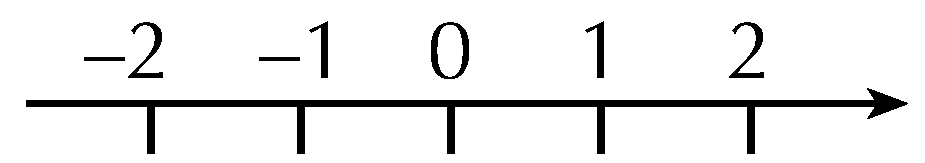
\includegraphics[height=10mm]{./pics/integers.pdf}
	\begin{block}{Die Menge $\ZZ$}
		\begin{itemize}
			\item Die Elemente von $\ZZ$ sind die Zahlen
				\begin{align*}
					0,\ \pm1,\ \pm2,\ \pm3,\ \ldots
				\end{align*}
			\item Diese werden die \emph{ganzen Zahlen} genannt.
			\item Sie k\oe nnen auf einer Zahlengerade abgetragen werden.
		\end{itemize}
	\end{block}
\end{frame}

\begin{frame}\frametitle{Vergleich}
\begin{block}{}
\begin{itemize}
\item $x=y$ ``$x$ ist gleich $y$''
\item $x<y$ ``$x$ ist kleiner als $y$''
\item $x>y$ ``$x$ ist gr\oe\ss er als $y$''
\item $x\leq y$ ``$x$ ist kleiner oder gleich $y$''
\item $x\geq y$ ``$x$ ist gr\oe\ss er oder gleich $y$''
\end{itemize}
\end{block}
\end{frame}
	
\begin{frame}\frametitle{Die nat\ue rlichen Zahlen}
\begin{itemize}
	\item $\NN=\{z\in\ZZ:z>0\}$ hei\ss t die Menge der \emph{nat\ue rlichen Zahlen}
	\item $\NN_0=\NN\cup\{0\}$
\end{itemize}
\end{frame}

\begin{frame}\frametitle{Die Grundrechenarten}
	\begin{block}{}
		\begin{itemize}
			\item \emph{Addition:} $x+y$\\
				werden mehrere Zahlen $x_1,x_2,\ldots,x_k$ addiert, verwenden wir die Schreibweise
				\begin{align*}
					x_1+x_2+\cdots+x_k=\sum_{i=1}^kx_i
				\end{align*}
			\item \emph{Multiplikation:} $x\cdot y$\\
				werden Zahlen $x_1,x_2,\ldots,x_k$ multipliziert, schreibt man
				\begin{align*}
					x_1\cdot x_2\cdot \enspace\cdots\enspace\cdot x_k=\prod_{i=1}^kx_i
				\end{align*}
			\item \emph{Subtraktion:} $x-y$\\
				{\itshape In der Mathematik ist diese Schreibweise \ue blich; die sonst im deutschsprachigen Raum vorherrschende Schreibweise $x./.y$ wird in der Vorlesung nicht verwendet.}
		\end{itemize}
	\end{block}
\end{frame}

\begin{frame}\frametitle{Rechenregeln}
	\begin{block}{}
		F\ue r alle $x,y,z\in\ZZ$ gelten folgende Regeln.
		\begin{description}
			\item[Assoziativgesetz] $(x+y)+z=x+(y+z)$ und $(x\cdot y)\cdot z=x\cdot(y\cdot z)$
			\item[Kommutativgesetz] $x+y=y+x$ und $x\cdot y=y\cdot x$
			\item[Neutrales Element] $0+x=x$ und $1\cdot x=x$
			\item[Distributivgesetz] $x\cdot(y+z)=x\cdot y+x\cdot z$
		\end{description}
	\end{block}
\end{frame}

\begin{frame}\frametitle{Das Dezimalsystem}
\begin{block}{}
Jede ganze Zahl $z$ kann in der Form
	\begin{align*}
		z=s\cdot\sum_{i=0}^\ell a_i\cdot 10^i
	\end{align*}
	dargestellt werden mit
\begin{itemize}
\item $s=\pm1$,
\item $z_i\in\{0,1,2,3,4,5,6,7,8,9\}$,
\item $\ell\geq0$
\end{itemize}
\end{block}
\end{frame}

\begin{frame}\frametitle{Das Dezimalsystem}
\begin{block}{Beispiel}
Die ganze Zahl $z=-127$ schreiben wir als
	\begin{align*}
		z=(-1)\cdot\bc{7\cdot 10^0+2\cdot 10^1+1\cdot 10^2}
	\end{align*}
\begin{itemize}
\item $s=-1$,
\item $z_0=7$, $z_1=2$, $z_2=1$
\item $\ell=2$
\end{itemize}
\end{block}
\end{frame}

\begin{frame}\frametitle{Die Addition}
\begin{block}{Wie addiert man positive Zahlen?}
\begin{itemize}
\item Seien
	\begin{align*}
		y&=\sum_{i=0}^\ell y_i\cdot 10^i,&
		z&=\sum_{i=0}^\ell z_i\cdot 10^i&&(0\leq y_i,z_i<10)
	\end{align*}
	Dezimaldarstellungen zweier positiver ganze Zahlen.
\item wir addieren $y,z$ stellenweise mit \Ue bertrag
\item f\ue r $\ell=0$ ist das einfach
\end{itemize}
\end{block}
\end{frame}

\begin{frame}\frametitle{Die Addition}
\begin{itemize}
\item f\ue r $\ell\geq1$ addiere zun\ae chst
\begin{align*}
	y'&=\sum_{i=0}^{\ell-1} y_i\cdot 10^i,&
	z'&=\sum_{i=0}^{\ell-1} z_i\cdot 10^i
	\end{align*}
\item bezeichne das Ergebnis mit
	\begin{align*}
		s'&=\sum_{i=0}^\ell s_i'\cdot 10^i&&(0\leq s_i'<10)
	\end{align*}
\item jetzt addiere die drei Ziffern $y_\ell,z_\ell,s_\ell'$:
\begin{align*}
	y_\ell+z_\ell+s_\ell'=s_\ell+10\cdot s_{\ell+1}&&(0\leq s_\ell,s_{\ell+1}<10)
\end{align*}
\item mit $s_i=s_i'$ f\ue r $i<\ell$ erhalten wir dann das Gesamtergebnis
	\begin{align*}
		y+z=\sum_{i=0}^{\ell+1} s_i\cdot 10^i
	\end{align*}
\end{itemize}
\end{frame}

\begin{frame}\frametitle{Die Addition}
\begin{block}{Beispiel}\centering
	\begin{tabular}{r|lll}
		$y$&&9&8\\
		$z$&&7&9\\
		\Ue bertrag&1&1&\\\hline
		$s$&1&7&7
\end{tabular}
\end{block}
\end{frame}

\begin{frame}\frametitle{Die Subtraktion}
\begin{block}{Subtraktion via Addition}
\begin{itemize}
\item Seien zwei Dezimalzahlen gegeben:
	\begin{align*}
		y&=\sum_{i=0}^\ell y_i\cdot 10^i,&
		z&=\sum_{i=0}^\ell z_i\cdot 10^i&&(0\leq y_i,z_i<10)
	\end{align*}
\item Wir nehmen an, da\ss\ $y\geq z>0$.
\item Um die Differenz $y-z$ zu berechnen, rechnen wir
	\begin{align*}
		\bc{(10^{\ell+1}-z)+y}-10^{\ell+1}=\bc{\bc{ (10^{\ell+1}-1)-z }+y+1}-10^{\ell+1}
	\end{align*}
\end{itemize}
\end{block}
\end{frame}

\begin{frame}\frametitle{Die Subtraktion}
	\hfill\emph{$y-z=\bc{\bc{ (10^{\ell+1}-1)-z }+y+1}-10^{\ell+1}$}
	\begin{block}{Subtraktion via Addition}
		\begin{itemize}
			\item Die Subtraktion $ (10^{\ell+1}-1)-z $ ist einfach, denn
				\begin{align*}
					10^{\ell+1}-1=\underbrace{999\cdots 9}_{\mbox{$\ell+1$ mal}}
				\end{align*}
			\item daher k\oe nnen wir ziffernweise Subtrahieren
			\item die letzte Subtraktion $\cdots -10^{\ell+1}$ ist ebenfalls einfach: wir l\oe schen lediglich die f\ue hrende Dezimalstelle
		\end{itemize}
	\end{block}
\end{frame}

\begin{frame}\frametitle{Die Subtraktion}
	\hfill\emph{$y-z=\bc{\bc{ (10^{\ell+1}-1)-z }+y+1}-10^{\ell+1}$}
	\begin{block}{Beispiel}
		\begin{itemize}
			\item $y=256$, $z=64$; also $\ell=2$
			\item $10^{\ell+1}-1-z=999-z=935$
			\item $(10^{\ell+1}-1-z)+y=935+256=1191$
			\item $(10^{\ell+1}-1-z)+y+1=1192$
			\item $\bc{\bc{ (10^{\ell+1}-1)-z }+y+1}-10^{\ell+1}=1192-1000=192$
		\end{itemize}
	\end{block}
	{\itshape Dieses Verfahren ist \ae quivalent zur Schulmethode!}
\end{frame}

\begin{frame}\frametitle{Die Multiplikation}
\begin{block}{Zerlegung in Dezimalziffern}
\begin{itemize}
\item Wieder seien zwei Dezimalzahlen gegeben:
	\begin{align*}
		y&=\sum_{i=0}^\ell y_i\cdot 10^i,&
		z&=\sum_{i=0}^\ell z_i\cdot 10^i&&(0\leq y_i,z_i<10)
	\end{align*}
\item Wir berechnen das Produkt $y\cdot z$ mit der Formel
	\begin{align*}
		y\cdot z=\sum_{i=0}^\ell\sum_{j=0}^\ell y_i\cdot z_j\cdot 10^{i+j}
	\end{align*}
\item Die Multiplikationen $y_iz_j$ sind einfach (`kleines Einmaleins')
\item Multiplizieren mit $10^{i+j}$ ist auch einfach (Stellen verschieben)
\end{itemize}
\end{block}
\end{frame}

\begin{frame}\frametitle{Zusammenfassung}
\begin{itemize}
	\item die ganzen Zahlen $\ZZ=\{0,\pm1,\pm2,\pm3,\dots\}$
	\item Addition, Subtraktion, Multiplikation
	\item Addition und Subtraktion erfordern eine \emph{lineare} Zahl elementarer Operationen
	\item das Multiplikationsverfahren ben\oe tigt eine \emph{quadratische} Zahl elementarer Operationen
\end{itemize}
\end{frame}

\end{document}
